\documentclass[9pts]{article}
\usepackage[utf8]{inputenc}
\usepackage[top=2.5cm, bottom=2.5cm, left=1.5cm, right=1.5cm]{geometry}

\usepackage{listings}
\usepackage{color}
\usepackage{graphicx}
\usepackage{caption}

\definecolor{mygreen}{rgb}{0,0.6,0}
\definecolor{mygray}{rgb}{0.5,0.5,0.5}
\definecolor{mymauve}{rgb}{0.58,0,0.82}

\lstset{
  backgroundcolor=\color{white},   % choose the background color; you must add \usepackage{color} or \usepackage{xcolor}; should come as last argument
  basicstyle=\footnotesize,        % the size of the fonts that are used for the code
  breakatwhitespace=false,         % sets if automatic breaks should only happen at whitespace
  breaklines=true,                 % sets automatic line breaking
  captionpos=b,                    % sets the caption-position to bottom
  commentstyle=\color{mygreen},    % comment style
  deletekeywords={...},            % if you want to delete keywords from the given language
  escapeinside={\%*}{*)},          % if you want to add LaTeX within your code
  extendedchars=true,              % lets you use non-ASCII characters; for 8-bits encodings only, does not work with UTF-8
  frame=single,	                   % adds a frame around the code
  keepspaces=true,                 % keeps spaces in text, useful for keeping indentation of code (possibly needs columns=flexible)
  keywordstyle=\color{blue},       % keyword style
  language=Octave,                 % the language of the code
  morekeywords={*,...},            % if you want to add more keywords to the set
  numbers=left,                    % where to put the line-numbers; possible values are (none, left, right)
  numbersep=5pt,                   % how far the line-numbers are from the code
  numberstyle=\tiny\color{mygray}, % the style that is used for the line-numbers
  rulecolor=\color{black},         % if not set, the frame-color may be changed on line-breaks within not-black text (e.g. comments (green here))
  showspaces=false,                % show spaces everywhere adding particular underscores; it overrides 'showstringspaces'
  showstringspaces=false,          % underline spaces within strings only
  showtabs=false,                  % show tabs within strings adding particular underscores
  stepnumber=2,                    % the step between two line-numbers. If it's 1, each line will be numbered
  stringstyle=\color{mymauve},     % string literal style
  tabsize=2,	                   % sets default tabsize to 2 spaces
  title=\lstname                   % show the filename of files included with \lstinputlisting; also try caption instead of title
}

\title{[4AI02] Projet C++: Algorithme de Dijkstra}
\author{
  Géhère, Kévin\\
  \texttt{kevin.gehere@sorbonne-universite.fr}
  \and
  Fraillon, Vincent\\
  \texttt{vincent.fraillon-maison@sorbonne-universite.fr}
}

\begin{document}
\maketitle

\section{Introduction}
Le but de ce projet est de vous montrer de manière sommaire mais réaliste une utilisation réelle de la Standard Template Librairy (\emph{STL}).
Pour ce faire, vous allez implémenter l'algorithme de Dijkstra,
un algorithme qui vise à évaluer le coût minimal pour aller d'un point A à un point B.

Cet algorithme peut s'appliquer sur des graphes orientés, modèle auquel plusieurs réseaux de transports sont disponibles (RATP, SNCF, routes, etc). Cet algorithme est également une porte d'entrée pour le domaine de la théorie des graphes, ou pour la résolution du problème du plus court chemin, vu également dans l'unité d'enseignement [4AI04] Intelligence artificielle.

\begin{figure}[h]
   \centering
   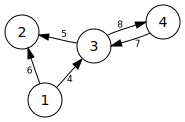
\includegraphics{directed_graph.pdf}
   \caption{\label{directed_graph} Exemple de graphe orienté}
\end{figure}

La développement est dans la plupart des cas simplement un moyen de faire fonctionner une idée simple au travers d'un programme, ou bien complexe au travers d'une association de programmes.
La plus grande difficulté d'un développeur vient donc plus du fait de trouver l'environnement le mieux adapté pour faire fonctionner cette idée que l'idée elle même,
qui est souvent déjà présente et fonctionnelle (cas évident des mathématiques).
Par analogie, il faut poser le sol avant de pouvoir marcher. \\

Dans le cadre de ce projet, l'accent sera mis sur les structures.\\

Si vous souhaitez contextualiser le projet vous pouvez vous mettre dans la situation suivante.
Vous êtes membre d'une start-up qui veut se lancer sur le marché de la vente de données de trafic.
Pour ce faire il vous faut implémenter une algorithme capable de planifier des temps de parcours au moyen d'une heuristique fixe ou dynamique.
Une base de données réaliste et fiable pour le tester est réquis pour établir la validité de son implémentation et du cadre dans lequel va naître le projet.
L'algorithme de Dijkstra et la base de données libre de la RATP sont des choix logiques car robustes.
Après concertation, un contrat est écrit pour juger des fonctionnalités minimums ne fréinant pas l'évolutivité de la solution.
%Vous recevez le cahier des charges des commerciaux qui vous demande les fonctionnalités minimum du projet que vous traduisez en contrat de programmation.

\section{Objectifs}
Un contrat en programmation est le fait qu'une classe hérite d'une classe mère virtuelle pure sans implémentation.
Ce principe permet de rajouter des fonctionnalités à une classe sans l'altérer et en garantissant sont appel via un pointeur sur le contrat.
Si la classe respecte le contrat, peu importe ses autres fonctionnalités, elle garantit d'avoir implémenter les fonctionnalités du contrat. \\

La class \emph{Generic\_class} aura cet objectif pour vous évaluer (voir annexes).
Vous devrez dériver de cette classe pour créer la votre.


\section{Charte d'écriture}
Dans le but d'évaluer vos connaissances le mieux possible, ce projet est décomposé en étapes clés.
Une charte d'écriture vous est imposée, comme dans les entreprises et les projets communs de manière générale. \\

Celle charte, imposée (donc obligatoire) est légère, énoncée dans un ordre quelconque:
\begin{itemize}
\item \textbf{Utilisation des drapeaux de compilation -Wall -Wextra -Werror -O3 de g++} afin de garantir le respect de l'implémentation dans les normes C++, et d'optimiser la compilation;
\item \textbf{Utilisation des fonctionnalités du C++ 11 maximum} afin d'utiliser les ressources du cours; %https://msdn.microsoft.com/fr-fr/library/hh567368.aspx
\item \textbf{Proscription de l'utilisation des outils d'allocation dynamique} : \emph{new}, \emph{new[]}, \emph{delete} et \emph{delete[]}, afin d'optimiser la sécurité, la lisibilité, et de tirer parti du concept \emph{RAII} : l'acquisition d'une ressource est une initialisation;
\item \textbf{Mémoire dynamique via les conteneurs de la \emph{STL}} ou les outils de \emph{memory} comme par exemple \emph{std::unique\_ptr}, celui-ci étant inutile dans le cadre du projet;
\item \textbf{Indentation parfaite du code source du programme} afin de garantir la lisibilité et de prévenir les erreurs d'implémentation;
\item \textbf{Minimisation de duplication du code source du programme} afin d'éviter le dangereux copier-coller est les graves problèmes de maintenance qui s'y accompagne;
\item \textbf{Obligation d'utilisation de la convention \emph{snake\_case}}, avec des noms de fonctions en \emph{verbe\_complément}, afin de garantir la lisibilité du code;
\item \textbf{Tout type créé commence par une majuscule}; % kézako
\item \textbf{Les constantes déclarées via \emph{define} sont écrites intégralement en majuscules}; on parlera ici de \emph{SCREAMING\_SNAKE\_CASE};
\item \textbf{Membres de classes appelés via \emph{this}} afin de répèrer facilement ces appels;
\item \textbf{Variables d'entrées précédées d'un underscore \emph{\_}}, également pour faciliter la lecture;
\item \textbf{Variables locales neutres}; % kézako
\item \textbf{Utilisation du mot clef \emph{const} lorsque l'entrée ne doit pas être modifiée}, afin de garantir ses droits d'accès en lecture/écriture;
\item \textbf{Utilisation systématique de référence ou de pointeur lors du passage d'un objet}, pour des raisons évidentes de passage par référence;
\item \textbf{Respect du typage lors des comparaisons au moyen de \emph{static\_cast$<$Type$>$(var)} si nécessaire}.
\end{itemize}

\pagebreak

\section{Temps et notation}

Quatre séances de 4H chacune sont mis à votre disposition pour réaliser ce projet.
Lors de chaque séance nous metterons l'accent sur une nouvelle étape à réaliser. Le rythme n'est pas imposé étant donné que vous pouvez soumettre à tout moment lors de la période du projet.
Des programmes de test vous seront fournis afin d'évaluer votre code et d'estimer son niveau d'accomplissement.
Les étapes seront:
\begin{enumerate}
\item Surcharge des operateurs de flux pour les données et la dérivation du contrat ($+$3pts $=>$ 3$/$20)
\item Lecture \& affichage des stations ($+$3pts $=>$ 6$/$20)
\item Lecture \& affichage des connections ($+$3pts $=>$ 9$/$20)
\item Génération \& affichage du graphe ($+$4pts $=>$ 13$/$20)
\item Estimation du meilleur chemin ($+$8pts $=>$ 21$/$20)
\item (BONUS) heuristique dynamique ($+$6pts $=>$ 27$/$20)
\end{enumerate}

La non-conformité de votre code à l'un de ces critères de la charte d'écriture pour noter le projet vous fera perdre un nombre conséquent de points, à partir de deux points (2/20) par critère non respecté. Ceux-ci seront vérifiés de manière automatique.\\

Tout point au dessus de 20 sera utilisé comme bonus pour les 4 premiers TPs. \\

\section{Soumission et autoévaluation}

La soumission du projet se fera sur l'espace Moodle dédié. Vous pourrez y soumettre un nombre illimité de projet, la dernière soumission écrasant les précédentes.

FIXME : Ici la description des outils d'auto-évaluation

\appendix
\clearpage
\section{Generic\_class.hpp}
\lstinputlisting[language=C++]{../src/Generic_class.hpp}

\end{document}
